\section{The NEXT Infrastructures}
\label{sec.infra}
%%%%%%%%%%

\subsection{Working platform, seismic pedestal and lead castle}

Figure \ref{fig.WP} shows the layout of the experimental area. All the systems are deployed on  $11 \times 11 \mathrm{m^2}$~ working platform, made of Tramex (figure \ref{fig.WPP}). The NEW detector is hosted inside a lead castle and sitting in a seismic pedestal (figure \ref{fig.LCWN}). The lead castle is made of lead blocks placed into a steel frame. The blocks are organised in a staggered structure to maximise the amount of lead seen by the external radiation. Additional steel sheets (made of radiopure steel-Ti alloy) provide the needed rigidity to avoid creep. The total weight of the lead is about 58 tons. 
The seismic pedestal is a frame with rectangular beams and 8 isolator seismic blocks. The pedestal is designed to swing without breaking in the event of earthquakes two orders of magnitude larger than the maximum earthquake recorded in the area. 


\begin{figure}[hpt!]
    \bigskip
    \begin{center}\leavevmode
        \rotatebox{0}{
        \includegraphics[width=0.7\textwidth, ]{img2/WorkingPlatform.png}}
        \caption{\textit{Layout of the NEXT working platform.}}
        \label{fig.WP}
    \end{center}
\end{figure}

\begin{figure}[hpt!]
    \bigskip
    \begin{center}\leavevmode
        \rotatebox{0}{
        \includegraphics[width=0.7\textwidth, ]{img2/PictureWP.png}}
        \caption{\textit{A picture of the NEXT working platform (April, 2016).}}
        \label{fig.WPP}
    \end{center}
\end{figure}

%
%
%\begin{figure}[hpt!]
%    \bigskip
%    \begin{center}\leavevmode
%        \rotatebox{0}{
%        \includegraphics[width=\textwidth, ]{GasSystemAndInfrastructures/IMG/F2.png}}
%        \caption{\textit{The NEXT working platform, empty}}
%        \label{fig:F2:F2}
%    \end{center}
%\end{figure}
%


\begin{figure}[hpt!]
    \bigskip
    \begin{center}\leavevmode
        \rotatebox{0}{
        \includegraphics[width=0.7\textwidth, ]{img2/LeadCastleWithNew.png}}
        \caption{\textit{The lead castle in open position. The NEW apparatus sits on top of the seismic pedestal, which is anchored to the floor via isolating seismic blocks.}}
        \label{fig.LCWN}
    \end{center}
\end{figure}

%\begin{figure}[hpt!]
%\centering
%\includegraphics[height=8cm]{img/SeismicPedestal.pdf}
%\caption{A 3D view of the Seismic Pedestal (SP).} \label{fig:seismicPedestal3D}
%\end{figure}
%


%\begin{figure}
%\centering
%\includegraphics[height=12cm]{img/InfraStruc.pdf}
%\caption{The NEXT infrastructures: (a) The pressure vessel, hosting the detector; (b) the lead castle shield in its open configuration; (c) seismic platform; (d) working platform; (e) gas purification system; (f) emergency gas vent tank; (g) data acquisition system; (h) other systems.} \label{fig:Infrastructure}
%\end{figure}
%
%\begin{figure}
%\centering
%\includegraphics[height=12cm]{img/InfraStruc_2.pdf}
%\caption{The NEXT-100 infrastructures (top view) showing the overall dimensions of the installation.} \label{fig:Infra2}
%\end{figure}


\subsection{Gas system}

\begin{figure}[hpt!]
    \bigskip
    \begin{center}\leavevmode
        \rotatebox{0}{
        \includegraphics[width=\textwidth, ]{img2/GasSystem.png}}
        \caption{\textit{Schematics of the NEW/NEXT Gas System.}}
        \label{fig.GasSystem}
    \end{center}
\end{figure}

The goal of the gas system, common to the NEW and NEXT-100 detectors is to purify the xenon, reducing the traces of gases such as ${\rm O_2, CO_2,CO, H_2, N_2, CH_4}$~ and water vapour to less than one part per billion (ppb). Both NEW and NEXT-100 will operate with natural xenon and enriched xenon. The gas will be maintained at room temperature and 10--15 bar pressure inside the detector(s). The gas system has been designed to avoid significant losses of xenon under all foreseeable circumstances.

%\begin{figure}[hpt!]
%    \bigskip
%    \begin{center}\leavevmode
%        \rotatebox{0}{
%        \includegraphics[width=\textwidth, ]{img/Gas2.png}}
%        \caption{\textit{Drawing showing the main components of the NEXT gas sytem.}}
%        \label{fig.gas2}
%    \end{center}
%\end{figure}

Figure \ref{fig.GasSystem} shows a schematics of the gas system. Its main components are:  

\begin{itemize}
\item Emergency recovery system.
\item Pressure vessel (NEW or NEXT-100). 
\item Compressor (recirculation pump).
\item Purification loop (hot and cold getters).
\item Cryo-recovery system.
\item Argon/xenon bottles.
\item Pipes.
\item Control System.
\end{itemize}

The pipes are all plumed together using 1/2'' and 1'' stainless tube and flexible hoses where mechanical insulation is required. The initial operation of NEW is foreseen to 10 bar, with the possibility to operate at 15--20 bar in 2017. The nominal operation pressure of NEXT-100 is 15 bar. 

\subsubsection*{Emergency recovery tank and ancillary systems}

\begin{figure}[hpt!]
    \bigskip
    \begin{center}\leavevmode
        \rotatebox{0}{
        \includegraphics[width=0.55\textwidth, ]{img2/GasER.png}}
        \caption{\textit{Emergency Recovery section of the Gas System}}
        \label{fig.GER}
    \end{center}
\end{figure}


\begin{figure}[hpt!]
    \bigskip
    \begin{center}\leavevmode
        \rotatebox{0}{
        \includegraphics[width=10cm ]{img2/NEXT100AsRecoveryVessel.png}}
        \caption{\textit{The NEXT-100 pressure vessel operating as Emergency Recovery Tank.}}
        \label{fig.N100}
    \end{center}
\end{figure}

\begin{figure}[hpt!]
    \bigskip
    \begin{center}\leavevmode
        \rotatebox{0}{
        \includegraphics[width=0.45\textwidth, ]{img2/PUMP1.png}
        \includegraphics[width=0.45\textwidth, ]{img2/CartenValve.png}
        }
        \caption{\textit{Left:a picture of the vacuum pump (PUMP1) used to keep the recovery tank at a 
        nominal pressure of $10^{-5}$~mbar. The pump is sitting under the working platform. Right: a picture of
        the Carten valve used to separate the pressure side from the vacuum side in the gas system.}}
        \label{fig.P1}
    \end{center}
\end{figure}


The emergency recovery section of the gas system (figure \ref{fig.GER}) is designed to recover gas into a recovery tank in the event of over pressure in the gas system. During the operation of NEW, the existing pressure vessel of the NEXT-100 experiment (a tank with a volume of 2.560 m$^3$~ made of 316Ti alloy and with CE certification for operation at 15 bar) is reused as recovery tank (figure \ref{fig.N100}). In order to guarantee that gas is dumped into the recovery tank in the event of an over-pressure, the tank is kept during normal operations at $10^{-5}$~mbar. This is done by pumping the tank with the vacuum pump PUMP1 (figure \ref{fig.P1}--left panel)
through a pneumatic-activated guillotine valve (GV1), certified to separate pressure from 
vacuum zones ((figure \ref{fig.P1}--right panel). A second  manual valve GV2 acts as a backup. A pressure gauge (PG1) and a vacuum gauge (VG1) measure the pressure and vacuum in the recovery tank. A bursting disk installed in the recovery tank (BD1) will break at 5 bar, avoiding any over-pressure in the system. Notice that a pressure of 10 bar in the NEW vessel translates into a pressure of $\sim$1 bar in the recovery tank, and therefore 5 bar provides a wide tolerance margin.   
%A second disk, BD7, will break at 3 bar. The disk function is to avoid an over pressure over 30 bar in the gas system. In practice, BD7 is relevant only in case that BV1 is opened by mistake when there is pressure in the purification loop. 

%In normal operations, the vacuum pump (PUMP1) is pumping the recovery tank and GV1 is opened. The valve is automatically controlled by the Slow Control System and to be open needs a pneumatic pressure of 4.5-5 bar and a voltage of 24 VDC. This implies that the valve closes in failure (electrical of pneumatic shutdown at the experiment or the LSC). Also, if an emergency condition (need to recover the gas) arises, PUMP1 is turned off and GV1 closes. Emergency conditions are normally triggered by excess pressure in the NEW pressure vessel. In this case, the Carten Valve opens up and as GV2 is always open, the gas will evacuate to the tank through the safety evacuation line.A second pneumatic valve, SV6 is controlled by the Slow Control System and will open up in the event of excess pressure. If both the Carten valve and SV6 fail, disk BD2 will burst at 13 bar. 

\subsubsection*{Pressure vessel}

\begin{figure}[hpt!]
\centering
\includegraphics[height=6cm]{img2/PVGS.png}
\caption{A diagram of the pressure vessel section of the gas system.} \label{fig.pvgs}
\end{figure}

Figure \ref{fig.pvgs} shows the pressure vessel section of the gas system. Currently, the pressure vessel is that of NEW, 
a tank with a volume of 0.169 m$^3$~ fabricated with a radiopure steel-titanium alloy (316Ti) and certified to operate up to 20 bar. Inside the pressure vessel there is region (call the pressure side) held at high pressure (10--15 bar) and a region held at modest vacuum $10^{-5}--10^{-6}$~mbar (called the vacuum side). The two regions are separated by a sealing copper plate (called the mother-can), which is described with more detail in section \ref{sec.new}. 

To reach the desired vacuum level in the vacuum side, PUMP2 is switched on. In the event of a breach between the
pressure and the vacuum side PUMP2 is switched off by the Slow Control System. A bursting disk (BD3) will break at 3 bar, preventing the PMTs from being damaged, and the gas will be evacuated to the emergency recovery tank. A mass spectrometer (also called RGA, after the initials Residual Gas Analyser)
detects the partial pressure of gas in the vacuum side.


\subsubsection*{Recirculation compressor}

%\begin{figure}[hpt!]
%\centering
%\includegraphics[height=12cm]{img/Pump.pdf}
%\caption{Schematics of the SERA recirculation compressor, chosen by NEXT.} \label{fig:pump}
%\end{figure}

\begin{figure}[hpt!]
\centering
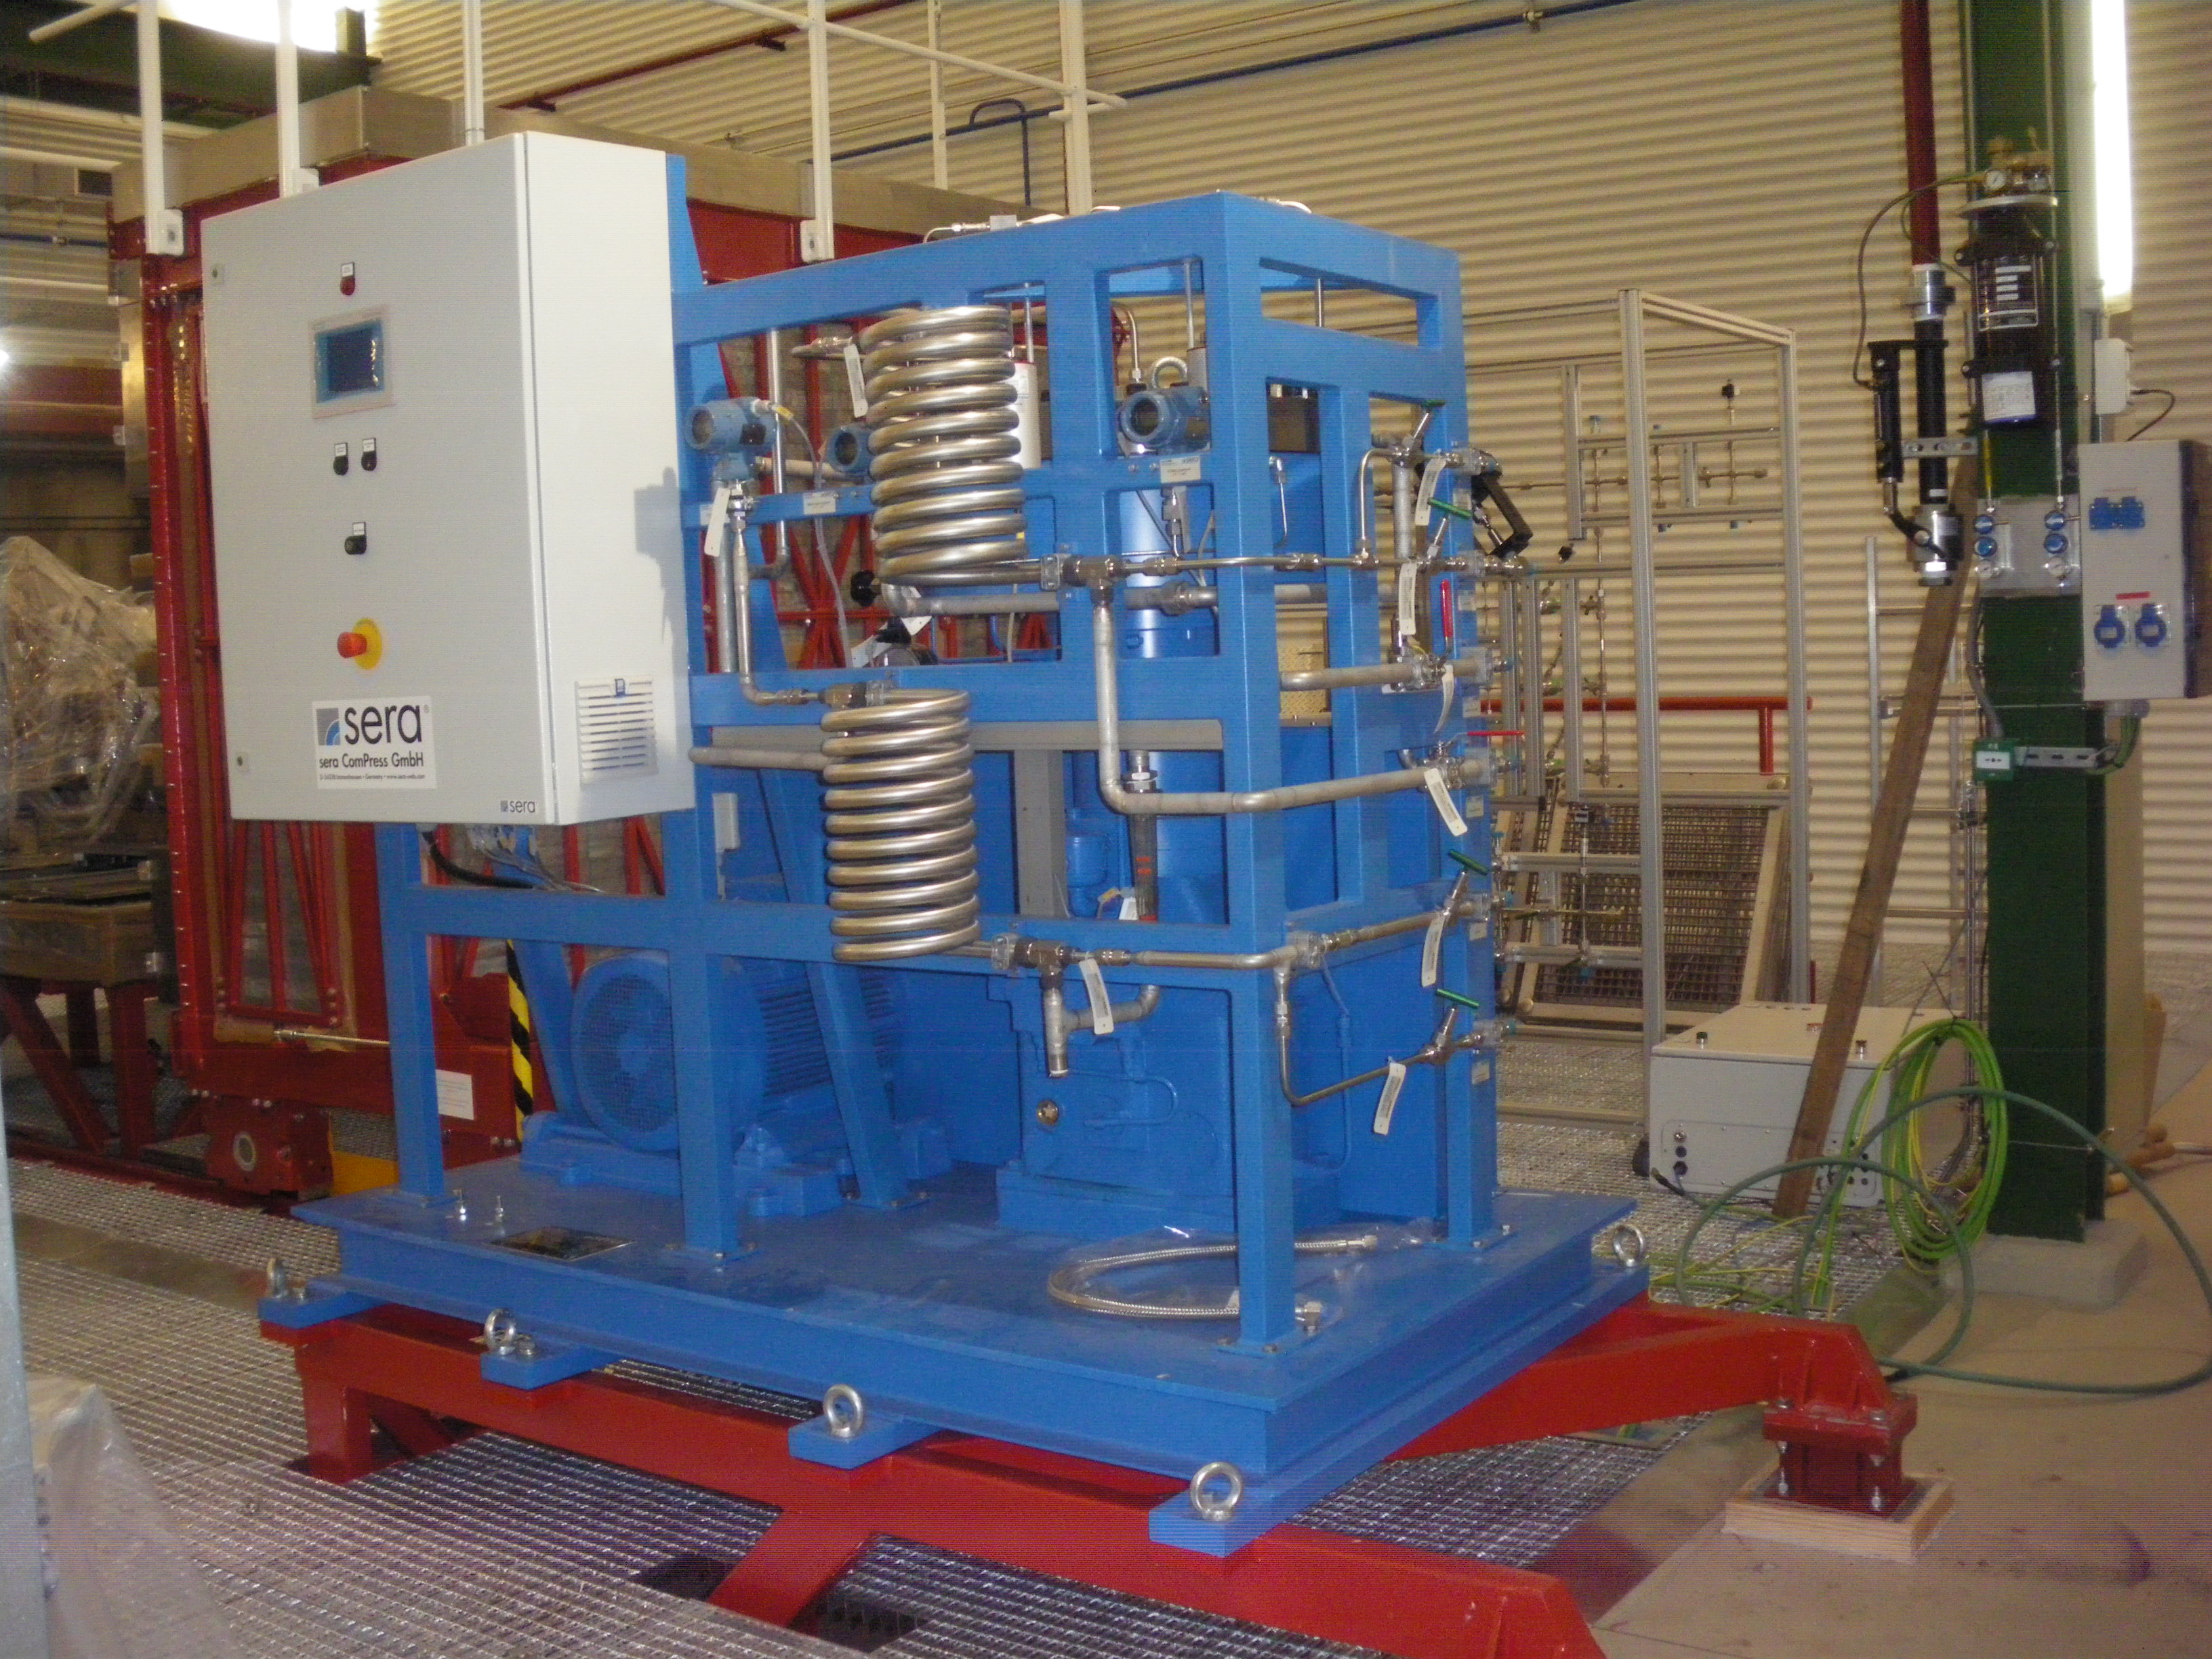
\includegraphics[height=8cm]{img2/Compressor.png}
\caption{A picture of the compressor.} \label{fig.sera}
\end{figure}

The most vulnerable component of the gas system is the compressor, which acts as a re-circulation pump. The enriched xenon is very expensive and therefore the pump to move the gas through the re-circulation loop must have sufficient redundancy to minimise the probability of failure and leakage. Furthermore, to preserve the purity of the gas all metal to metal seals must be used. 

Figure \ref{fig.sera} shows a picture of the compressor chosen for NEXT, manufactured by the SERA company, in Germany. The pump is made with metal-to-metal seals on all the wetted surfaces. The gas is moved through the system by a triple stainless steel diaphragm, ensuring a negligible probability of catastrophic failure (gas liberated to the atmosphere). Between each of the diaphragms there is a sniffer port to monitor for gas leakages. In the event of a leakage, automatic emergency shutdown can be initiated. 

\subsubsection*{Getters}

\begin{figure}[hpt!]
\centering
\includegraphics[height=8cm]{img2/HotGetter.png}
\includegraphics[height=8cm]{img2/ColdGetters.png}
\caption{Top: The PS4-MT50 SAES hot getter. Bottom: a detail of the gas system with the cold getters already installed.} \label{fig:getter}
\end{figure}


Hot and cold getters (figure \ref{fig:getter}) are used to purify the gas. The gas is circulated first through cold getters in order to eliminate water vapor, as well as other electron negative (oxygen and carbon dioxide) impurities. Once the gas is sufficiently clean the hot getter is switched on to remove nitrogen and methane and further purify the gas to less than 1 ppb. 

\subsubsection*{Recirculation loop and cryo-recovery }

\begin{figure}[hpt!]
\centering
\includegraphics[height=8cm]{img2/Recirculation.png}
\caption{An scheme of the recirculation loop and cryo-recovery part of the gas system.} \label{fig.ct}
\end{figure}

\begin{figure}[hpt!]
    \bigskip
    \begin{center}\leavevmode
        \rotatebox{0}{
        \includegraphics[width=8cm]{img2/CryoBottle.png}}
        \caption{\textit{The cryo-recovery system consists on a large bottle sitting inside an open Dewar. Cooling the bottle with liquid nitrogen reclaims the xenon circulating in the system.  }}
        \label{fig.CB}
    \end{center}
\end{figure}

Figure \ref{fig.ct} shows the recirculation loop. The gas enter the system from the pressure bottle, through a regulator and circulates through cold and/or hot getters ( \ref{fig:getter}), under the action of the compressor 
(figure \ref{fig.sera}). To recover the gas in normal conditions a bottle sitting inside an open Dewar (figure \ref{fig.CB}) is used. 

\subsubsection*{Summary}
 
The needed infrastructures for the NEXT experiment have been completed during 2015 and the first quarter of 2016. The gas system is now in the final commissioning phase, and ready to pass the tests needed for underground operation certification in the next few weeks. Start-of-operations is foreseen for May, 2016. 
